\documentclass[tikz,border=2pt]{standalone}
\usepackage{amsmath,amssymb}
\usetikzlibrary{arrows.meta}
\begin{document}
% (s,S) = (2,8) policy, lead time l = 1, demands 2,3,1,4,0,3,2,5,1,2: end-of-period inventory levels
% I_k' = 6,3,2,-2,4,1,-1,1,0,5. A period is ready when I_k' >= 0 (green, including I_9' = 0);
% periods 4 and 7 end with backlog, so the ready rate over these ten periods is 8/10 = 0.8.
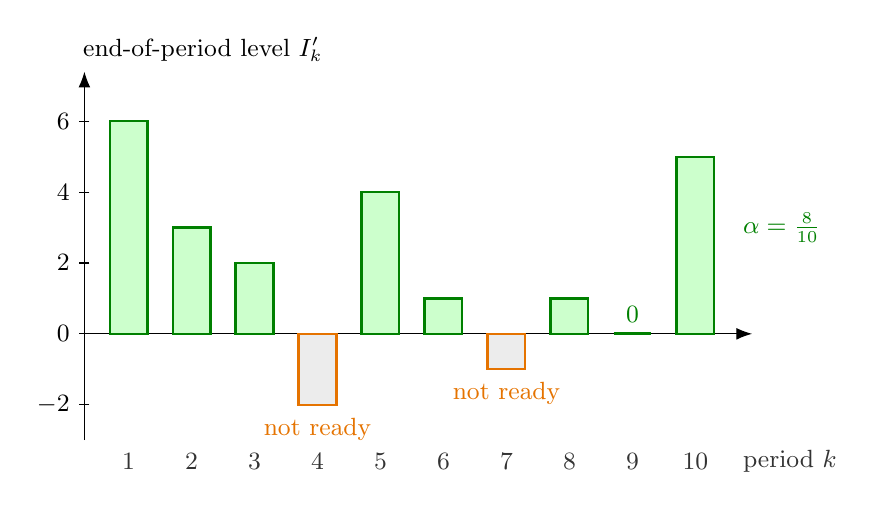
\begin{tikzpicture}[font=\small, >={Latex[length=2mm]}, x=0.8cm, y=0.45cm]
  \draw[->] (0.3,0) -- (10.9,0);
  \draw[->] (0.3,-3) -- (0.3,7.4) node[anchor=south west, xshift=-4pt] {end-of-period level $I_k'$};
  \foreach \v in {-2,0,2,4,6} {\draw (0.38,\v) -- (0.22,\v) node[left] {$\v$};}
  \foreach \k/\v in {1/6,2/3,3/2,5/4,6/1,8/1,10/5}
    {\fill[green!20] (\k-0.3,0) rectangle (\k+0.3,\v); \draw[green!50!black, thick] (\k-0.3,0) rectangle (\k+0.3,\v);}
  \draw[green!50!black, very thick] (8.7,0) -- (9.3,0);
  \node[green!50!black, anchor=south] at (9,0.05) {$0$};
  \foreach \k/\v in {4/-2,7/-1}
    {\fill[gray!15] (\k-0.3,0) rectangle (\k+0.3,\v); \draw[orange!90!black, thick] (\k-0.3,0) rectangle (\k+0.3,\v);}
  \foreach \k in {1,...,10} {\node[gray!40!black] at (\k,-3.6) {$\k$};}
  \node[gray!40!black, anchor=west] at (10.6,-3.6) {period $k$};
  \node[orange!90!black, anchor=north] at (4,-2.1) {not ready};
  \node[orange!90!black, anchor=north] at (7,-1.1) {not ready};
  \node[green!50!black, anchor=west] at (10.6,3) {$\alpha=\frac{8}{10}$};
\end{tikzpicture}
\end{document}
